% \begin{figure}
%     \centering
%     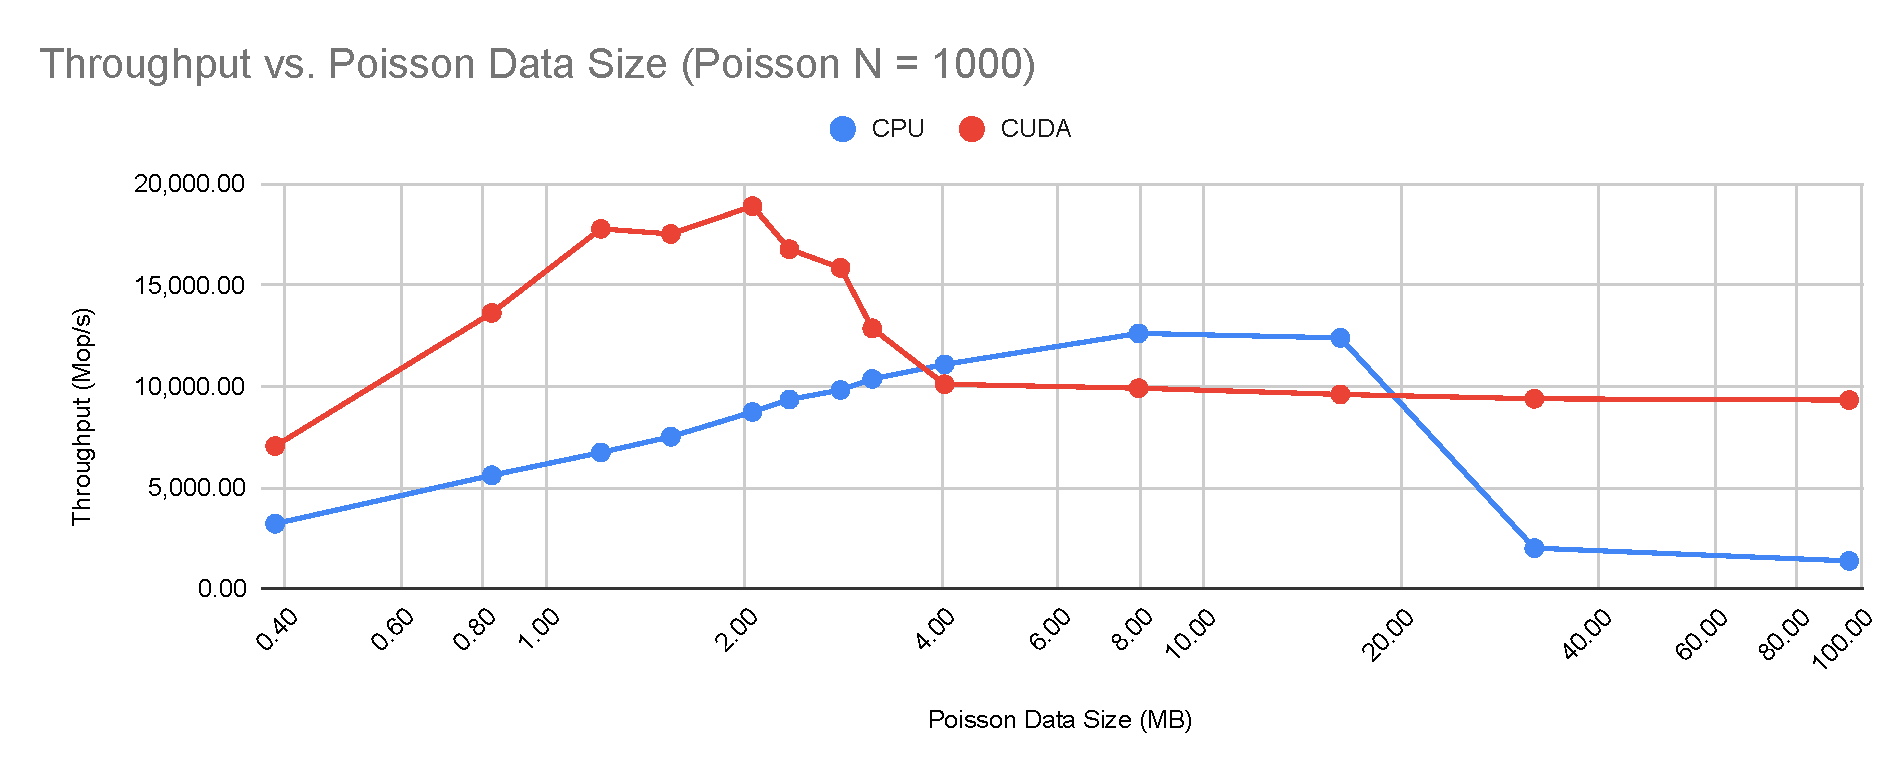
\includegraphics[width=\linewidth]{Ch62Results/figures/temp_throughput_over_size.pdf}
%     \caption{Simulation Throughput for CPU and CUDA as required data size increases.}
%     \label{fig:results:throughput_over_size}
% \end{figure}

\begin{figure}
    \centering
    \begin{tikzpicture}
    \begin{axis}[
        title={Throughput vs. Poisson Data Size (N = 1000)},
        ylabel={Throughput (\si{\giga\op\per\second})},
        xlabel={Poisson Data Size (\si{\mega\byte})},
        ymin=0, ymax=20000,
        xmin=0.35, xmax=128,
        xmode=log,
        xtick={0.4,0.8,1.2,1.6,2.0,4.0,8.0,16.0,32.0,64.0,128.0},
        scaled y ticks=base 10:-3,
        ytick scale label code/.code={},
        log basis x={2},
        log ticks with fixed point,
        width=\linewidth,
        height=15em,
        axis x line=bottom,
        axis y line=left,
    ]
    \addplot table [x=cache, y=cpu, col sep=space, ignore chars={\,}] {Ch62Results/figures/data/throughput_cache.csv};
    \addlegendentry{CPU};
    \addplot table [x=cache, y=cuda, col sep=space, ignore chars={\,}] {Ch62Results/figures/data/throughput_cache.csv};
    \addlegendentry{CUDA};
    \end{axis}
    \end{tikzpicture}
    % \caption{Simulation Throughput for CPU and CUDA as required data size increases}
    \caption{Simulation Throughput for CPU and CUDA vs Poisson cache size}
    \label{fig:results:throughput_over_size}
\end{figure}
